

\newcolumntype{P}[1]{>{\centering\arraybackslash}p{#1}}

\section{Experiments}
\label{sec:Experiments}

Our experiments study \name\ in Apache SystemDS\footnote{All code and experiments are available open source in Apache SystemDS (\url{https://github.com/apache/systemds}) and our reproducibility repository (\url{https://github.com/damslab/reproducibility}).} in comparison with uncompressed operations (ULA), compressed linear algebra (CLA)~\cite{ElgoharyBHRR16, ElgoharyBHRR18} in Apache SystemML, and different data types in TensorFlow. We evaluate a variety of micro benchmarks, end-to-end ML algorithms, and hyper-parameter tuning; with local, distributed, and hybrid runtime plans.

\subsection{Experimental Setting}
\label{sec:setup}

\textbf{Hardware Setup:}
Our local and distributed experiments use a scale-out cluster of $1+6$ ($1+11$) nodes,
each having a single AMD EPYC 7443P CPU at $2.85$\,GHz (24 physical/48 virtual cores),
$256\gb$ DDR4 RAM at 3.2\,GHz, $1\times 480\gb$ SATA SSD,
$8\times 2\tb$ SATA HDDs (data) and Mellanox ConnectX-6 HDR/200\,Gb Infiniband. 
We use Ubuntu 20.04.1, OpenJDK Java 11.0.13 with JVM arguments \texttt{-Xmx110g -Xms110g -Xmn11g}, 
Apache Hadoop 3.3.4, and Apache Spark 3.2.0. The CLA baseline uses SystemML 1.2 with Spark 2.4 and equivalent configurations.
Some experiments marked with * were run on another cluster (for comparison) of $1+6$ nodes with AMD EPYC 7302 CPU at $3.0-3.3$~GHz (16/32 cores).
$128\gb$ DDR4 RAM at 2.933\,GHz, $2\times 480\gb$ SATA SSDs (system/home), $12\times 2\tb$ HDDs (data), and $2\times 10\text{Gb}$ Ethernet.

\textbf{Datasets:}
Since compression is strongly data-dependent, we exclusively use the real datasets shown in Table~\ref{tab:data}. This selection includes dense, sparse, and ultra-sparse datasets with common data characteristics.
All reported sizes and compression ratios refer to the size in memory using a sparsity threshold of 0.4 for uncompressed matrices.
US\,Census \cite{uci} is further used in an encoded form with binning/one-hot encoding for numerical, and recoding/one-hot encoding for categorical features, resulting in an increase from 68 to 378 columns, and the increased sparsity from $0.43$ to $0.18$, but with negligible change of the size in memory.
For large-scale experiments, we use a replicated versions of US\,Census\,Enc (up to 128x) which is roughly $290\gb$ and after densifying operations more than $950\gb$.
The Spark default configuration uses a storage fraction of 0.5, which gives an aggregate cluster memory of $6 \cdot 105\gb \cdot 0.5 = 315\gb$.
That way, we scale to data sizes that require I/O per iteration in uncompressed representation.

\begin{table}[!t]
	\centering \setlength\tabcolsep{15.2pt}
	\caption{\label{tab:data}Datasets {\normalfont($n$ Rows, $m$ Columns, $sp$ Sparsity)}.}
	\vspace{-0.4cm}
	\begin{tabular}{rrrrr}
		\toprule
		\multicolumn{1}{c}{\textbf{Dataset}} & $n$ ($\text{nrow}(\mat{X})$) & $m$ ($\text{ncol}(\mat{X})$) & \multicolumn{1}{c}{$sp$} & \multicolumn{1}{c}{Size} \\
		\midrule
		Airline78 \cite{airline}             & \num{14462943}               & 29                           & 0.54                     & $3.4\gb$                 \\ %3355402928
		Amazon \cite{amazon,HeM16}           & \num{8026324}                & \num{2330066}                & 1.2e-6                   & $1.22\gb$                \\ %1220001352
		Covtype \cite{uci}                   & \num{581012}                 & 54                           & 0.22                     & $127\mb$                 \\ %128635964
		Mnist1m \cite{infimnist}             & \num{1000000}                & 784                          & 0.25                     & $2.46\gb$                \\ %2461000104
		US\,Census \cite{uci}                & \num{2458285}                & 68 (378)                     & 0.43 (0.18)              & $1.34\gb$                \\ %1337307192
		US\,Census 128x                      & \num{314660480}              & 68 (378)                     & 0.43 (0.18)              & $289.5\gb$               \\ % 2261750120 * 128 = 289504015360
		\bottomrule
	\end{tabular}
\end{table}

\subsection{Compression Performance}

We first investigate the compression process itself in terms of compression times, compression ratios, and the influence of workload characteristics.

\begin{table} [!t] \setlength\tabcolsep{11.7pt}
  \vspace{-0.4cm}
	\caption{\label{tab:compressionTimes} Local Compression Times [Seconds] and Ratios.}
	\vspace{-0.4cm}
	\begin{tabular}{r|rr|rr|rr}
    \toprule
    \textbf{Dataset} & \multicolumn{2} {c|}{\textbf{CLA}}                            & \multicolumn{2}{c|}{\textbf{\name-Mem}} & \multicolumn{2}{c}{\textbf{\name}}                                                                                        \\
                     & \multicolumn{1} {c}{time}                                     & \multicolumn{1} {c|}{ratio}             & \multicolumn{1} {c}{time}          & \multicolumn{1} {c|}{ratio} & \multicolumn{1} {c}{time} & \multicolumn{1} {c}{ratio} \\
    \midrule
    Airline78        & \numprint{9.34} sec                                           & \numprint{10.22}                        & \numprint{1.74} sec                & \numprint{8.61}             & \numprint{2.08} sec       & \numprint{7.94}            \\
    Amazon           & \multicolumn{2} {c|}{\numprint{ 37.6} \textit{hours Crash}  } & \numprint{8.54} sec                     & \numprint{1.73}                    & \numprint{  3.77} sec       & \textit{Abort}                                         \\
    Covtype          & \numprint{1.10} sec                                           & \numprint{13.79}                        & \numprint{0.84} sec                & \numprint{14.24}            & \numprint{1.23} sec       & \numprint{13.99}           \\
    Mnist1m          & \numprint{7.25} sec                                           & \numprint{7.14}                         & \numprint{4.57} sec                & \numprint{6.09}             & \numprint{17.50} sec      & \numprint{4.41}            \\
    US Census        & \numprint{5.15} sec                                           & \numprint{35.38}                        & \numprint{1.16} sec                & \numprint{29.60}            & \numprint{1.15} sec       & \numprint{27.35}           \\
    US Census Enc    & \numprint{27.48} sec                                          & \numprint{41.03}                        & \numprint{5.78} sec                & \numprint{38.46}            & \numprint{6.54} sec       & \numprint{29.46}           \\
    \bottomrule
\end{tabular}


\end{table}

\textbf{Compression Ratios:} Starting with local single-node matrix compression, we compare \name~ optimized for memory (\name-Mem) and for workload (\name) with the existing CLA framework \cite{ElgoharyBHRR16,ElgoharyBHRR18}. The used workload is a fixed cost summary of left matrix multiplications that leads to extensive co-coding of columns. Table~\ref{tab:compressionTimes} shows the compression times and ratios for all datasets, where the ratios are calculated from the sizes of in-memory representations.
We attribute the minor differences to published CLA compression ratios \cite{ElgoharyBHRR18} (Airline78 7.44, Covtype 18.19, US\,Census 35.69) to different data preparation and sparse memory estimates.
Compared to CLA, \name yields worse compression ratios except for CovType, where \name's co-coding finds other column groups and uses new encoding types.
The lower compression ratios are due to the tuning for operations performance rather than size, and in practice, moderate absolute differences of large compression ratios have only little impact on size.
For example, compressing a $1\gb$ input with ratio 7 versus 6 yields only a difference of ~$24\mb$.
The Amazon dataset is an interesting case, where CLA runs out of memory due to group memoization during co-coding ($>2.7\cdot10^{12}$ pairs of columns). In contrast, \name~ aborts the compression early because the estimated total costs exceed the costs of ULA. Optimizing for memory in \name~ yields a low compression ratio for Amazon because of object overheads per column group, which do not exist in ULA's CSR representation.

\textbf{Compression Times:}
Table~\ref{tab:compressionTimes} further shows the compression times for all datasets.
% \name~ generally reduces compression times when optimizing for size (up to ~8x) and cost (up to ~3.7x), which make compression easier to amortize.
% The speed difference in \name-Mem US\,Census\,Enc is due to a reduction of the Grouping phase from 27 to 2.7 seconds.
\name~ generally reduces compression times when optimizing for size (up to ~4.7x) and cost (up to ~4.2x), which makes compression easier to amortize.
The speed difference in \name-Mem US\,Census\,Enc is due to a reduction of the grouping phase from 19 to 2.4 seconds.
When using workload-aware compression with a fixed cost summary that causes more grouping and compression,
only MNIST and US\,Census have significantly slower compression compared to optimizing for memory.
MNIST is slow because combining column groups have a large number of distinct values (each column contains up to 256 distinct values, and three columns together has up to $256^3$ distinct tuples).

\begin{table} [!t] \setlength\tabcolsep{10pt}
	\caption{\label{tab:sparkComp}Spark RDD Compression {\normalfont(Data: US\,Census\,Enc)}.}
	\vspace{-0.4cm}

	\begin{tabular}{r|cr|cr|c}
\toprule
          & \multicolumn{2} {c|}{\textbf{\name-Mem}} & \multicolumn{2} {c|}{\textbf{\name}} &                          \\
Blocksize & Ratio                                    & Total Size                           & Ratio & Total Size & ULA \\
\midrule
1K   	 &	\numprint{8.94} &	\numprint{225.58} MB &	\numprint{7.83} &	\numprint{257.36} MB &	\numprint{2.02} GB    \\
2K   	 &	\numprint{15.1} &	\numprint{143.49} MB &	\numprint{10.9} &	\numprint{198.55} MB &	\numprint{2.17} GB    \\
16K   	 &	\numprint{26.6} &	\numprint{81.68} MB &	\numprint{23.3} &	\numprint{93.36} MB &	\numprint{2.17} GB    \\
64K   	 &	\numprint{29.9} &	\numprint{72.74} MB &	\numprint{23.4} &	\numprint{92.96} MB &	\numprint{2.17} GB    \\
256K   	 &	\numprint{30.5} &	\numprint{71.22} MB &	\numprint{24.5} &	\numprint{88.70} MB &	\numprint{2.17} GB    \\
\bottomrule
\end{tabular}

\end{table}

\textbf{Compression Ratio Spark:}
For distributed operations, matrices are represented as Spark resilient distributed datasets (RDD) \cite{ZahariaCDDMMFSS12}---i.e.,
distributed collections of key-value pairs---with values being fixed-size matrix blocks of size $b \times b$ (except boundary blocks).
These blocks are compressed independently with separate compression plans and dictionaries.
The default block size is $b=1\text{K}$ ($8\mb$ dense blocks), but sparsity and compression warrant larger blocks.
Table~\ref{tab:sparkComp} varies this block size $b$ for US\,Census, and reports the size of \name-Mem, \name, and uncompressed (ULA) RDDs (from Spark's cached RDD-infos).
With small blocks, there is larger variability of compression, and increasing block sizes give better ratios while also stabilizing the resulting compression plans.
Overall, \name~ yields good compression ratios even with small $b$ and approaches local compression ratios with larger $b$.
For the remaining experiments, we use a block size of $b=16\text{K}$.


\subsection{Operations Performance}
\label{sec:OperationPerformance}

In a second series of micro-benchmarks, we compare the runtime of \name~ with ULA and CLA operations.
While CLA was designed for operations performance close to uncompressed and benefits from keeping large datasets in memory,
\name~ aims to improve performance more generally, even for in-memory settings and keep performance stable even if the input data is densified.
% Here, we focus on common aggregations, element-wise matrix-vector operations, small sequences of operations, as well as left, right, and transpose-self matrix multiplications.
We compare using both original and densified by simply adding 1 to all cells.

\textbf{Aggregations:} Figure~\ref{exp:sum} shows the results for computing the aggregate $\text{sum}(\mat{X})$. CLA processes each column group in parallel, aggregates individual sums, and combines them into the result. ULA uses multi-threading with sequential scans of row partitions.
By memorizing the frequencies of tuples, \name~ executes purely on the column group dictionaries without scanning their indexes because of memoization.
Without memoization, the execution time increase according to the complexity of scanning the index structures.
For instance, we observed no penalty in case of Census\,enc, while 60x performance drop in Census for \name.
When densifying, in Figure~\ref{exp:sumDense}, CLA and \name~ retain their performance while ULA's performance worsen.
For column aggregations (Figure~\ref{exp:colSum} and \ref{exp:colSumDense}), CLA is slower than ULA because CLA's DDC colSums is not specialized for DDC1 and DDC2 and thus, performs a lookup of dictionary values for each encoded cell.

\begin{figure}[!t]
	\centering
	\subfigure[Sum Original]{\label{exp:sum}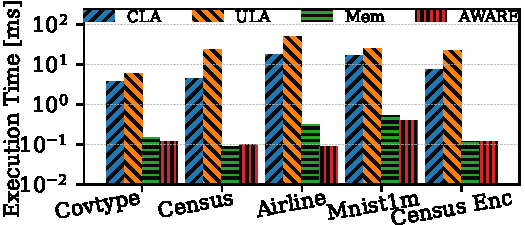
\includegraphics[width= 0.47 \linewidth]{\source/microbenchmark/ua/sum_dams-so001.pdf}}\hfill
	\subfigure[Sum Dense]{\label{exp:sumDense}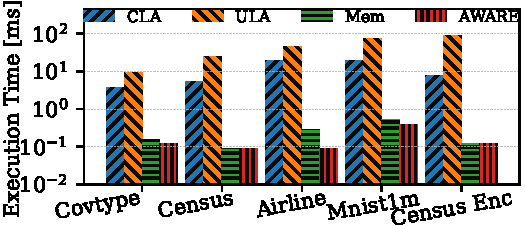
\includegraphics[width= 0.47 \linewidth]{\source/microbenchmark/ua/sum+_dams-so001.pdf}}\hfill~\vspace{-0.3cm}\\
	\subfigure[ColSums Original]{\label{exp:colSum}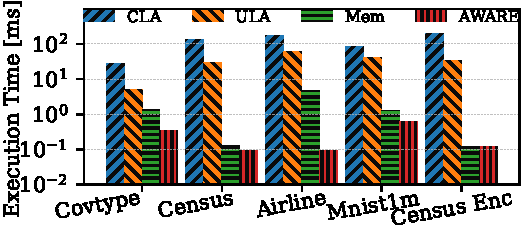
\includegraphics[width= 0.47 \linewidth]{\source/microbenchmark/ua/colsum_dams-so001.pdf}}\hfill
	\subfigure[ColSums Dense]{\label{exp:colSumDense}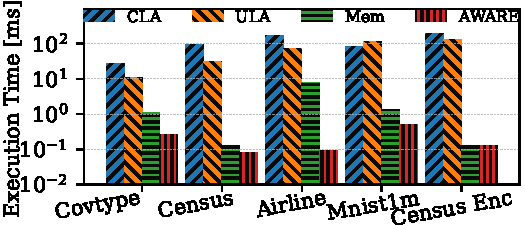
\includegraphics[width= 0.47 \linewidth]{\source/microbenchmark/ua/colsum+_dams-so001.pdf}}~\vspace{-0.4cm}\\
	% \subfigure[Plus Original]{\label{exp:plus}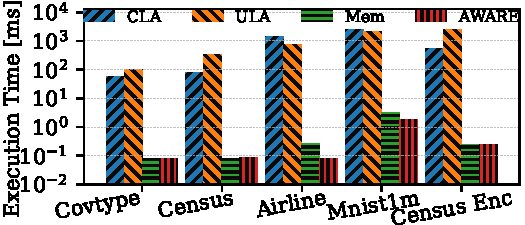
\includegraphics[width= 0.49 \linewidth]{\source/microbenchmark/sc/plus_dams-so001.pdf}}\hfill
	% \subfigure[Div Row-vector Dense]{\label{exp:divVectorDense}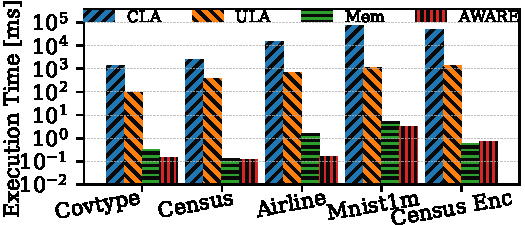
\includegraphics[width= 0.49 \linewidth]{\source/microbenchmark/ua/divvector+_dams-so001.pdf}}~\vspace{-0.3cm}\\
	\caption{\label{exp:opsua}Operations Performance Aggregate.}
	\Description{ microbenchmarks }
  \vspace{-0.4cm}
\end{figure}

\begin{figure}[!t]
	\subfigure[Plus Scalar, Original]{\label{exp:plus}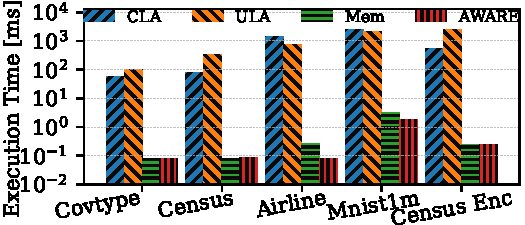
\includegraphics[width= 0.47 \linewidth]{\source/microbenchmark/sc/plus_dams-so001.pdf}}\hfill
	\subfigure[Div Row-vector, Dense]{\label{exp:divVectorDense}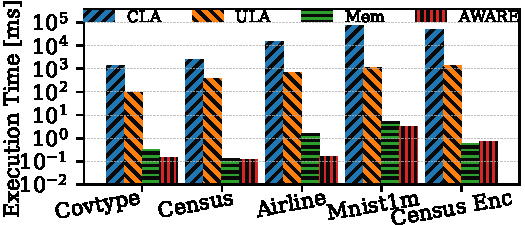
\includegraphics[width= 0.47 \linewidth]{\source/microbenchmark/ua/divvector+_dams-so001.pdf}}~\vspace{-0.4cm}\\
	\caption{\label{exp:opsscalar}Operations Performance Scalar.}
	\Description{ microbenchmarks }
\vspace{-0.4cm}
\end{figure}


% \textbf{Element-wise Operations:} Figure~\ref{exp:plus} shows the performance of adding a scalar value to each matrix cell. We observe extreme speedups of up to 4984x because \name\ avoids modifying dictionaries where possible. Figures~\ref{exp:divVectorDense} shows similar improvements for matrix-vector (column vector) element-wise operations. Specifically, we analyze $\mat{X}/\mat{v}$ on sparse and dense representations, where we chose division because it forces modifications of the dictionaries. We still see speedups of about three orders of magnitude (1766x).
\textbf{Element-wise Operations:} Figure~\ref{exp:plus} shows the performance of adding a scalar value to each matrix cell. We observe extreme speedups of up to \numprint{10766}x because \name\ avoids modifying dictionaries where possible. Figures~\ref{exp:divVectorDense} shows similar improvements for matrix-vector (row vector) element-wise operations. Specifically, we analyze $\mat{X}/\mat{v}$ on sparse (not shown) and dense representations, where we chose division because it forces modifications of the dictionaries. We still see speedups of about three orders of magnitude (\numprint{2047}x).

\textbf{Left Matrix Multiplication (LMM):}
Left, right, and transpose-self matrix multiplications are key operations in many ML algorithms.
In the following, we first evaluate these operations independently.
Figure~\ref{exp:LMM} shows the results of left matrix multiplications for all datasets, where the uncompressed left-hand-side has 16 rows.
CLA emulates this matrix-matrix multiplication via 16 vector-matrix multiplications.
We observe \name~ performance comparable to multi-threaded ULA (sparse and dense) with improvements
for Covtype, US\,Census, and US\,Census\,Enc,
but a moderate slowdown for Airlines and a significant slowdown for MNIST.
LMM also shows a major performance difference when optimizing for memory versus optimizing for operations, which is especially noticeable in US\,Census\,Enc.
In contrast, for datasets with smaller potential for co-coding like Airline, there is no difference.
Figure~\ref{exp:mmlscale} shows results on US\,Census\,Enc with varying number of rows in the left-hand-side.
CLA performs similar to \name~ at a single row, but when rows increase CLA's performance decrease to the same as ULA due to the lack of native matrix-matrix support.
CLA is worse at utilizing more threads, while \name~ and ULA scale better.
For ULA and \name-Mem, there is a change in parallelization strategies after 16 rows.
In contrast, \name~ yields between half and one order of magnitude speedups for all \#rows configurations.

\begin{figure}[!t]
	\subfigure[16 row LMM]{\label{exp:LMM}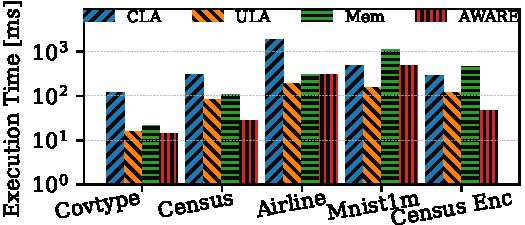
\includegraphics[width= 0.47  \linewidth]{\source/microbenchmark/mm/16_mml_dams-so001.pdf}}\hfill
	\subfigure[LMM Census Enc Scaling]{\label{exp:mmlscale}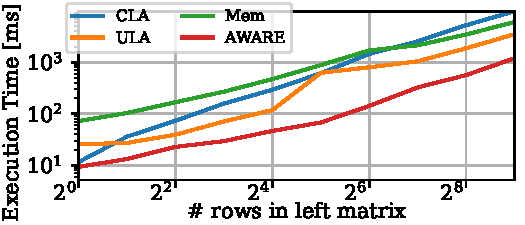
\includegraphics[width= 0.47  \linewidth]{\source/microbenchmark/mm/mml_census_dams-so001.pdf}}~\vspace{-0.4cm}\\

	\caption{\label{exp:opsLMM}Operations Performance Left Matrix Multiplication.}
	\Description{ microbenchmarks }
\end{figure}

\begin{figure}[!t]
	\subfigure[16 col RMM]{\label{exp:RMM}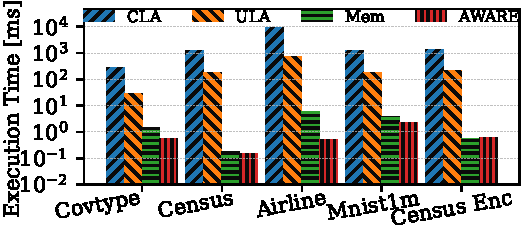
\includegraphics[width= 0.47  \linewidth]{\source/microbenchmark/mm/16_mmr_dams-so001.pdf}}\hfill
	\subfigure[RMM Census Enc Scaling]{\label{exp:mmrscale}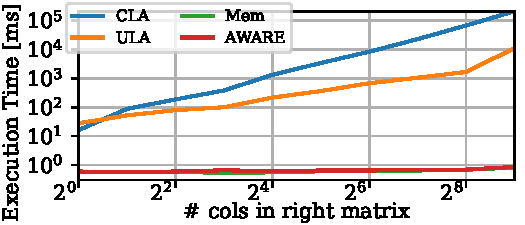
\includegraphics[width= 0.47  \linewidth]{\source/microbenchmark/mm/mmr_census_dams-so001.pdf}}~\vspace{-0.4cm}\\
	\caption{\label{exp:opsRMM}Operations Performance Right Matrix Multiplication.}
	\Description{ microbenchmarks }
	\vspace{-0.4cm}
\end{figure}

\textbf{Right Matrix Multiplication (RMM):}
In contrast to LMM, the right matrix multiplication creates outputs of overlapping column groups with a shallow copy of the index structures.
Figure~\ref{exp:RMM} shows the results for all datasets, where we observe \name~ speedups between
% 34x to 656x
53x to \numprint{1528}x
because of the deferred aggregation across column groups.
Figure~\ref{exp:mmrscale} then shows the scaling with increasing number of columns in the uncompressed right-hand-side.
CLA shows equal performance to uncompressed in the single column case but scales worse then ULA, again due to the lack of native matrix-matrix multiplication.
\name's RMM exhibits better asymptotic behavior due to its dictionary-centric operations,
% yielding speedups >$15000$x for 512 columns.
yielding speedups >\numprint{13000}x for 512 columns.

\begin{figure}[!t]
	\subfigure[TSMM Sparse]{\label{exp:tsmm}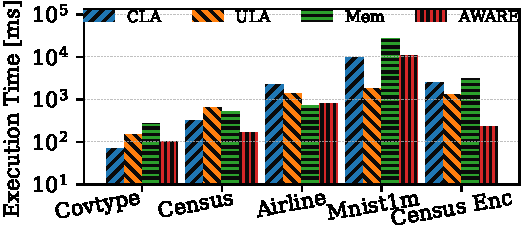
\includegraphics[width= 0.47  \linewidth]{\source/microbenchmark/ua/tsmm_dams-so001.pdf}}\hfill
	\subfigure[TSMM Dense]{\label{exp:tsmmDense}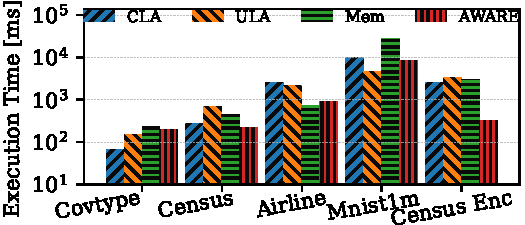
\includegraphics[width= 0.47  \linewidth]{\source/microbenchmark/ua/tsmm+_dams-so001.pdf}}~\vspace{-0.4cm}\\
	\caption{\label{exp:opsTSMM}Operations Performance Transpose Self Matrix Multiplication.}
	\Description{ microbenchmarks }
	\vspace{-0.4cm}
\end{figure}

\textbf{Transpose-Self Matrix Multiplication (TSMM):} Figures~\ref{exp:tsmm} and \ref{exp:tsmmDense} show the results of TSMM operations as used for computing PCA, direct-solve linear regression, as well as covariance and correlation matrices.
We observe speedups on all datasets except MNIST, where \name\ yields a substantial slowdown, especially for sparse inputs.
The TSMM performance is largely dependent on the number of column groups, their number of distinct items, and thus,
co-coding decisions. MNIST has a high number of columns, with high cardinality, and low correlation between columns.

\begin{figure}[!t]
	\subfigure[Scale and Shift Sparse]{\label{exp:scaleShift}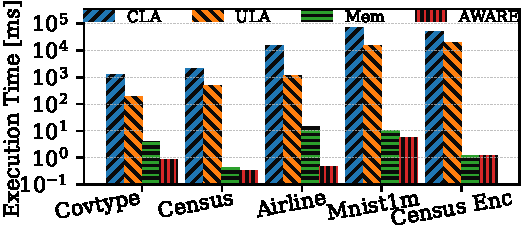
\includegraphics[width= 0.47  \linewidth]{\source/microbenchmark/ua/scaleshift_dams-so001.pdf}}\hfill
	\subfigure[Euclidean MinDist 16 Points Dense]{\label{exp:euclideanDense}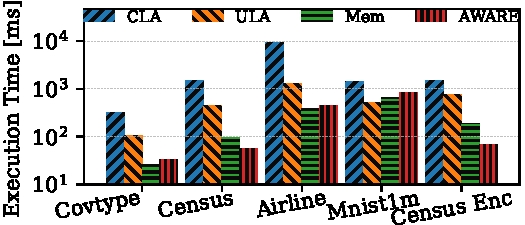
\includegraphics[width= 0.47  \linewidth]{\source/microbenchmark/mm/16_euclidean+_dams-so001.pdf}}~\vspace{-0.4cm}\\
	\caption{\label{exp:opsseq}Operations Performance Sequence.}
	\Description{ microbenchmarks }
\end{figure}

\textbf{Operation Sequences:}
As final micro benchmark use cases, we evaluate two sequences of operations. First, \emph{scale and shift} in Figure~\ref{exp:scaleShift}
performs a shifting $\mat{Y} = \mat{X} - (\text{colSums}(\mat{X})/\text{nrow}(\mat{X}))$ and scaling $\mat{Z} = \mat{Y} / \sqrt{\text{colSums}(\mat{Y}^2)/(\text{nrow}(\mat{Y})-1)}$.
This sequence is a common normalization step (standard-scaler) of the input data but has the negative side effect of densifying the input data.
% \name~ improves performance up to  a best case of 11924x. Second, we compute the minimum Euclidean distances via $\mat{D} = -2 * (\mat{X} \times t(\mat{C})) + t(rowSums(\mat{C}^2))$, followed by $\mat{d} = rowMins(\mat{D})$ (which forces a decompression from overlapping state). Here, $\mat{D}$ are the Euclidean distances of each row in \mat{X} to the coordinates \mat{C}. This expressions is used, for instance, in K-Means clustering. \name~ shows performance up to 14.5x faster compared to ULA in all cases except MNIST.
\name~ improves performance up to a best case of \numprint{15399}x. Second, we compute the minimum Euclidean distances via $\mat{D} = -2 * (\mat{X} \times \text{t}(\mat{C})) + \text{t}(\text{rowSums}(\mat{C}^2))$, followed by $\mat{d} = \text{rowMins}(\mat{D})$ (which forces a decompression from overlapping state). Here, $\mat{D}$ are the Euclidean distances of each row in \mat{X} to the centroids \mat{C}. This expressions is used, for instance, in K-Means clustering. \name~ shows performance up to 11.3x faster compared to ULA in all cases except MNIST.

\begin{table} [!t] \setlength\tabcolsep{17.4pt}
	\caption{\label{tab:expOverlap}RMM Overlap Sequence (Data: US\,Census\,Enc).}
	\vspace{-0.4cm}
	\begin{tabular}{r|r|r|r|r}
    \toprule
                   & \textbf{I/O}        & \textbf{Comp}        & \textbf{RMM}          & \textbf{Total}        \\
    \midrule
    SystemML - ULA & \numprint{0.84} sec & ---                  & \numprint{188.40} sec & \numprint{190.03} sec \\
    SystemML - CLA & \numprint{0.88} sec & \numprint{24.34} sec & \numprint{374.13} sec & \numprint{401.27} sec \\
    SystemDS - ULA & \numprint{0.81} sec & ---                  & \numprint{189.27} sec & \numprint{190.42} sec \\
    \name-No OL    & \numprint{0.76} sec & \numprint{3.97} sec  & \numprint{189.59} sec & \numprint{195.51} sec \\
    \name-Mem      & \numprint{0.80} sec & \numprint{8.00} sec  & \numprint{0.38} sec   & \numprint{9.72} sec   \\
    \name          & \numprint{0.78} sec & \numprint{3.93} sec  & \numprint{0.42} sec   & \numprint{5.69} sec   \\
    \bottomrule
\end{tabular}


\end{table}

\textbf{Overlap:} Leveraging the overlapping output from RMM without compaction shows significant improvements in Figures \ref{exp:RMM} and \ref{exp:opsseq}.
However, overlapping representations are most beneficial in chains of RMMs. Table \ref{tab:expOverlap} shows the end-to-end runtime for a sequence of $10$ RMM of size $k=512$, representative for processing $10$ fully-connected layers of size $512$ with no activation.
CLA is slower than ULA in this scenario because it is falling back to vector matrix compressed operations for the first multiplication.
\name~ with no overlapping is slower because the first right multiplication decompress, but it does show close to ULA performance.
% of its compression overhead, non-native matrix-matrix multiplications, decompressed intermediates and ULA operations after the first RMM.
%and finally because the subsequent uncompressed MM are worse at utilizing the cores
%dropping average cores utilized from $15.6$ to $8.6$ --> likely due to allocations.
\name~ with overlapping column groups push the compressed index structures through the entire chain of RMMs, improving performance irregardless of optimizing for memory or workload, with a slight advantage to workload.


\begin{table} [!b] \setlength\tabcolsep{8pt}
	\caption{ \label{tab:workload} \name \ Workload TOPS (Data: US\,Census\,Enc).}
	\vspace{-0.4cm}
	\begin{tabular}{r|rr|rrrr}
    \toprule
                   & \multicolumn{2} {c|}{\textbf{ULA}} & \multicolumn{4} {c}{\textbf{\name}}                                                                                                                  \\
    Op ($100\times$) & \multicolumn{1}{c}{TOPS}           & \multicolumn{1}{c|}{Time}           & \multicolumn{1}{c}{Est. TOPS} & \multicolumn{1}{c}{TOPS} & \multicolumn{1}{c}{Comp} & \multicolumn{1}{c}{Time} \\
    \midrule
    SUM & 3.38e+10  & \numprint{2.25} sec & 1.29e+05  & 1.14e+05 & \numprint{4.60} sec  & \numprint{0.08} sec \\
    SUM Dense & 1.90e+11  & \numprint{8.96} sec & 1.31e+05  & 1.14e+05 & \numprint{4.65} sec  & \numprint{0.07} sec \\
    RMM-256 & 2.81e+13  & \numprint{156.97} sec & 2.13e+07  & 1.94e+07 & \numprint{4.74} sec  & \numprint{0.25} sec \\
    LMM-256 & 4.28e+12  & \numprint{185.69} sec & 6.87e+11  & 7.14e+11 & \numprint{7.22} sec  & \numprint{53.76} sec \\
    TSMM & 6.32e+12  & \numprint{111.12} sec & 9.83e+11  & 9.98e+11 & \numprint{7.19} sec  & \numprint{16.91} sec \\
    ScaleShift & 7.47e+11  & \numprint{3216.21} sec & 4.08e+05  & 3.42e+05 & \numprint{4.89} sec  & \numprint{0.36} sec \\
    Euclidean-256 & 4.80e+13  & \numprint{308.85} sec & 8.61e+11  & 9.04e+11 & \numprint{7.87} sec  & \numprint{78.55} sec \\
    \bottomrule
    \end{tabular}

\end{table}

\textbf{Computation Cost:} Table \ref{tab:workload} shows the \name~ workload analysis of different micro benchmarks on Census\_Enc.
This experiment shows the estimated Theoretical Operations (TOPS), calculated from the cost vectors and compression schemes.
We compare the estimated TOPS for uncompressed operations (on the left) with \name's estimated TOPS extracted from the sample and co-coding decisions, as well as the estimated TOPS after compression (on the right). We observe that the estimated TOPS from the sample is close to the actual TOPS, indicating good estimation accuracy and thus, meaningful costs. We also show the compression time (Comp) and the runtime (Time) for executing 100 repetitions of the given operation (Op $100\times$). There are some micro benchmarks that show disproportionate scaling of runtimes compared to TOPS. With small execution times, moderate discrepancies are expected because of various unaccounted overheads in both ULA and \name. For TSMM and LMM, the differences are due to output allocation, memory bandwidth limitations, and index structure lookups. Although the runtime discrepancies are sub-par, we found that our TOPS estimation provides a good balance of simplicity and reflecting key differences relevant for compression. More sophisticated cost estimators are, however, interesting future work.

% \subsection{Computation Cost}
% Figure~\ref{exp:censusBreakdown} shows how optimizing for cost or memory changes the compression. Each plot is split into two parts: left the individual columns and right the co-coded column groups. First, the left plot shows cost in Tera Operations (TOPS), because FLOPs is not a good measure here since many operations are index lookups and bit shifting. We compare estimated and actual TOPS, which do not represent real instructions but abstract cost units our cost model is based on. Similar cost units can also be extracted for the uncompressed input and operations. Second, the right plot compares the estimated and actual size in memory when optimizing for size (\name-Mem). In both cases, the total score of a compression plan is the area under the curve. We see that co-coding reduces the number of column groups more when optimizing for computation cost---because it reduces the number operations---whereas when optimizing for size, co-coding decisions depend more on column correlations to be beneficial.

\subsection{End-to-End Algorithm Performance}
\label{sec:end-to-end}

% After having discussed the compression and operations micro-benchmarks,
% we can now turn to evaluating \name~ with workload-ware compression on end-to-end ML algorithms.
We use the following six algorithms to evaluate \name~ with workload-ware compression on end-to-end ML training:
K-Means for clustering;
principal component analysis (PCA) for dimensionality reduction;
multinomial (multi-class) logistic regression (MLogReg);
LM via conjugate gradient (lmCG), and via a direct solve method (lmDS) for linear regression;
as well as
l2-regularized support vector machines (L2SVM) for classification.
In theory, \name~ gives equal results to ULA but because of rounding errors in sequences of
FP64 operations and different parallelization strategies---present both, in ULA and \name---algorithms naturally execute with slight variations.
Therefore, algorithm parameters are set to ensure an equal number of iterations and operations.
We use the US\,Census\,Enc dataset and scale up by replication.
The replication maintains the statistics of the data,
and is not an issue for distributed execution, where blocks are compressed independently.
The local influence is limited to constant dictionary sizes, and replication is not actively exploited by \name.


\begin{table}[!t]
	\setlength\tabcolsep{10pt}
	\centering
	\caption{\label{tab:end2end}Workload-awareness on Local End-to-End Algorithms (Data: US\,Census\,Enc)}
	\vspace{-0.4cm}

	\begin{tabular}{r|r|rr|rr}
    \toprule
                     & \textbf{ULA}        & \multicolumn{2}{c|}{\textbf{\name-Mem}} & \multicolumn{2}{c}{\textbf{\name}}                                             \\
                     & Time                & Comp                                    & Time                               & Comp                & Time                \\
    \midrule
    \textbf{K-Means} &	\numprint{51.6} sec &	\numprint{4.2} sec &	\numprint{46.2} sec &	\numprint{6.2} sec &	\numprint{27.1} sec  \\
    \textbf{PCA}     &	\numprint{12.7} sec &	\numprint{4.0} sec &	\numprint{10.4} sec &	\numprint{6.0} sec &	\numprint{9.0} sec  \\
    \textbf{MLogReg} &	\numprint{32.0} sec &	\numprint{4.5} sec &	\numprint{32.5} sec &	\numprint{7.2} sec &	\numprint{26.0} sec  \\
    \textbf{lmCG}    &	\numprint{19.8} sec &	\numprint{5.0} sec &	\numprint{20.7} sec &	\numprint{6.4} sec &	\numprint{18.6} sec  \\
    \textbf{lmDS}    &	\numprint{15.6} sec &	\numprint{5.7} sec &	\numprint{15.5} sec &	\numprint{6.1} sec &	\numprint{14.3} sec  \\
    \textbf{L2SVM}   &	\numprint{38.9} sec &	\numprint{6.5} sec &	\numprint{45.2} sec &	\numprint{6.2} sec &	\numprint{36.5} sec  \\
    \bottomrule
    \end{tabular}
    

\end{table}%

\begin{table}[!t]
	\centering
	\setlength\tabcolsep{10pt}
	% \captionsetup{width=0.4\textwidth}
	\caption{\label{tab:expCLAEndToEnd}L2SVM (without scale\&shift, 60 iterations, Data: US\,Census\,Enc)}
	\vspace{-0.4cm}

	
\begin{tabular}{r|r|r|r|r||r}
    \toprule
                   & \multicolumn{4}{c||}{Local {\tiny(1x)}} & Distributed {\tiny(256x)}                                                                                   \\
    \midrule
                   & \textbf{I/O}                            & \textbf{Comp}             & \textbf{L2SVM}      & \textbf{Total}      & \multicolumn{1}{c}{ \textbf{Total}} \\

    \midrule
    SystemML - ULA & \numprint{1.6} sec                      & ---                       & \numprint{36.7} sec & \numprint{38.4} sec & \numprint{5689.6} sec               \\
    SystemML - CLA & \numprint{1.5} sec                      & \numprint{32.8} sec       & \numprint{31.7} sec & \numprint{66.0} sec & \numprint{4722.7} sec               \\
    SystemDS - ULA & \numprint{1.6} sec                      & ---                       & \numprint{19.3} sec & \numprint{20.9} sec & \numprint{2849.1} sec               \\
    \name-Mem      & \numprint{1.4} sec                      & \numprint{6.0} sec        & \numprint{21.3} sec & \numprint{28.7} sec & \numprint{2300.4} sec               \\
    \name          & \numprint{1.6} sec                      & \numprint{7.9} sec        & \numprint{15.9} sec & \numprint{25.3} sec & \numprint{2294.9} sec               \\
    \bottomrule
\end{tabular}


\end{table}%

\textbf{Local Execution:}
Table~\ref{tab:end2end} shows the results algorithms fit in-memory.
\name~ yields moderate but consistent improvements, or at worst (e.g. L2SVM, lmDS) comparable performance.
% Observing improvements of 36\% for MLogReg, 48\% for K-Means (iterative algorithms), and 27\% for PCA (non-iterative algorithm) is remarkably because this includes online compression. Underlying reasons are fast compression that is easier to amortize and redundancy exploiting operations.
Observing improvements on all algorithms most notably 19\% for MLogReg, 47\% for K-Means (iterative algorithms), and 29\% for PCA (non-iterative algorithm) is remarkably because this includes online compression.
Underlying reasons are fast compression that is easier to amortize and redundancy exploiting operations.
The algorithms L2SVM, lmCG, and lmDS all perform very close to ULA.

\textbf{CLA Comparison:} CLA is not included in Table \ref{tab:end2end} because it does not support scale\&shift and therefore would not execute efficiently.
For a fair comparison, we use the L2SVM algorithm from CLA \cite{ElgoharyBHRR18} (with minor modifications, e.g. 60 iterations not 100) and compare different configurations of CLA (in SystemML) and \name~ in Table~\ref{tab:expCLAEndToEnd}.
Both systems read and parse both train and test datasets (in binary), increasing I/O compared to the other experiments.
We observe that CLA compression is slower than \name~ optimizing for size or compute.
CLA does not outperform ULA in SystemML in local settings because the compression is not amortized.
In contrast, our ULA baseline is 1.9x faster, \name-Mem shows similar performance to CLA, and \name~ improves the relative training time (without compression and IO) by 2x over CLA, and 2.3x over ULA, but SystemDS ULA is the fastest end-to-end. 
Since CLA mostly focuses on large distributed datasets, we further compare CLA and \name~ on a larger sparse dataset (256x, which only partly fits in memory of 11 nodes). Table~\ref{tab:expCLAEndToEnd} (right) shows that SystemML CLA yields a moderate speedup, but \name~ achieves another 2x over SystemML CLA.
At this scale, \name~ optimizes for memory size and thus, the results \name~ and \name-Mem are similar.

\newcommand{\headendtoendtwo}{
	& \multicolumn{2}{c|}{\textbf{lmCG}}
	& \multicolumn{2}{c|}{\textbf{lmDS}}
	& \multicolumn{2}{c}{\textbf{L2SVM}} \\}


\newcommand{\headendtoendone}{
	& \multicolumn{2}{c|}{\textbf{K-Means}}
	& \multicolumn{2}{c|}{\textbf{PCA}}
	& \multicolumn{2}{c}{\textbf{MLogReg}} \\}

\newcommand{\subhead}{
	& \textbf{ULA}  & \textbf{\name} & \textbf{ULA} & \textbf{\name} & \textbf{ULA} & \textbf{\name} \\
}

\newcommand{\dist}{{\tiny$^D$}}


\begin{table} [!t] \setlength\tabcolsep{11.2pt}
	\caption{\label{tab:end2endSU}End-to-End Algorithms Hybrid Execution [Seconds] (Data: US\,Census\,Enc, $D$ .. Incl.\,Distributed\,Ops).}
	\vspace{-0.4cm}

	\begin{tabular}{r|rr|rr|rr}
    \toprule
    \headendtoendone
    \midrule
    \subhead
    \midrule
    1x    & \numprint{51.6}         & (\numprint{6}) \numprint{27.1}   & \numprint{12.7}       & (\numprint{6}) \numprint{9.4}   & \numprint{32.0}        & (\numprint{7}) \numprint{26.0}   \\
    8x    & \numprint{471.0}        & (\numprint{26}) \numprint{117.8} & \numprint{330.3}      & (\numprint{26}) \numprint{42.6} & \numprint{393.3}       & (\numprint{29}) \numprint{88.2}  \\
    16x   & \dist\numprint{484.3}   & (\numprint{48}) \numprint{183.9} & \dist\numprint{76.3}  & (\numprint{47}) \numprint{67.5} & \dist\numprint{570.3}  & (\numprint{58}) \numprint{144.2} \\
    32x   & \dist\numprint{1491.6}  & \dist\numprint{1496.3}           & \dist\numprint{70.3}  & \dist\numprint{61.2}            & \dist\numprint{671.5}  & \dist\numprint{629.9}            \\
    \midrule
    128x  & \dist\numprint{17819.0} & \dist\numprint{6298.0}           & \dist\numprint{137.0} & \dist\numprint{140.3}           & \dist\numprint{3502.9} & \dist\numprint{1710.6}           \\
    % MLogReg is not comparable with old results, since it is run with a different configuration of inner iterations (5 instead of 50 in the second cluster)
    *128x & \dist\numprint{33039.0} & \dist\numprint{11616.0}          & \dist\numprint{269.0} & \dist\numprint{259.0}           & \dist\numprint{50998.0} & \dist\numprint{8599.6}           \\
    \midrule
    \midrule
    \headendtoendtwo
    \midrule
    \subhead
    \midrule
    1x    & \numprint{19.8}         & (\numprint{6}) \numprint{18.6}   & \numprint{15.6}       & (\numprint{6}) \numprint{14.3}  & \numprint{38.9}        & (\numprint{6}) \numprint{36.5}   \\
    8x    & \numprint{366.2}        & (\numprint{26}) \numprint{60.6}  & \numprint{334.4}      & (\numprint{29}) \numprint{51.5} & \numprint{405.2}       & (\numprint{26}) \numprint{115.4} \\
    16x   & \dist\numprint{104.4}   & (\numprint{44}) \numprint{91.7}  & \dist\numprint{80.2}  & (\numprint{50}) \numprint{75.8} & \dist\numprint{252.6}  & (\numprint{56}) \numprint{195.5} \\
    32x   & \dist\numprint{264.6}   & \dist\numprint{105.3}            & \dist\numprint{91.5}  & \dist\numprint{70.8}            & \dist\numprint{433.2}  & \dist\numprint{479.4}            \\
    \midrule
    128x  & \dist\numprint{1611.4}  & \dist\numprint{242.6}            & \dist\numprint{175.9} & \dist\numprint{162.4}           & \dist\numprint{5286.9} & \dist\numprint{1904.5}           \\
    % last number (l2svm+) is not included since the iterations stopped at 34 iterations of the algorithm not 80 (altho it was converged.) this discrepancy is not in the new results.
    *128x & \dist\numprint{33090.0}  & \dist\numprint{469.0}            & \dist\numprint{365.9} & \dist\numprint{465.0}           & \dist\numprint{74016.0} & \dist\numprint{1060.0}           \\
    \bottomrule
\end{tabular}


\end{table}


\textbf{Hybrid Execution:} In between the local and distributed extremes, there are hybrid runtime plans, where the sparse input fits into memory
of the driver but after scale\&shift transformation, the transformed data does not fit in the driver and thus, generates distributed operations.
Table \ref{tab:end2endSU} show the results for replicated versions of US\,Census\,Enc (8x-32x).
Runs using distributed operations are marked with $D$ and local compression times are included in parenthesis.
These in-between scenarios are generally challenging in terms of evictions,
efficient exchange between local and distributed runtimes, as well as decisions on when to prefer distributed operations.
Most notable is this characteristic in ULA, which is sometimes faster for larger scales.
This is because the execution fits in memory for various instructions and therefore more or less instructions are executed distributed.
For instance in PCA, the number of distributed instructions grows from 16x to 32x to finally 128x.
Across all algorithms---except for a few instances---\name~ show consistent improvements, especially if we focus on computation time (without the compression time).

\textbf{Large-scale Execution:}
Finally, the last two rows (128x) show the primary compression scenario, where both
the sparse input and dense intermediate after transformation do not fit into local memory
and the dense intermediate exceeds aggregate cluster memory.
We still compile hybrid runtime plans but all operations on \mat{X} (and some derived intermediates) are distributed.
Since the data exceeds aggregate memory, iterative algorithms read in every iteration more than two thirds of \mat{X} from evicted partitions.
The 128x results refer to our primary cluster setup but with a different memory configuration (more executors and nodes, smaller \texttt{spark.memory.fraction}) in order to ensure stable results. For comparison, we also include previous results from our secondary cluster (128x*) using the same configuration as hybrid execution, which caused lost executors in some cases. Due to redundancy exploitation and good compression ratios---even on tiles (see Table~\ref{tab:sparkComp})---we observe large improvements of 2.8x for K-Means, 2x for MLogReg, 6.6x for lmCG, and 2.8x for L2SVM. In contrast, PCA and lmDS are non-iterative algorithms. On the secondary cluster, we observed up to 70x performance gains. The differences in relative improvements are due to faster networking and OS file system caching of evicted partitions due to more physical memory per node ($256\gb$ versus $128\gb$), which favors uncompressed (ULA) operations. 
 

\subsection{Additional Baseline - TensorFlow}

While ULA is the most important
baseline---within the same compiler and runtime--- we
% also compare with TensorFlow (TF) version 2.8.
also compare with TensorFlow (TF) version 2.12;
% In detail, we compare with TF version 2.8,
% as a widely used ML system with support for different data types and lossy compression.
We evaluated both TF and TF-AutoGraph \cite{abs-1810-08061}, but report numbers for TF-AutoGraph, which gave 1-5 sec faster execution times on average.
The workload is a simplified version of lmCG on US\,Census\,Enc, expressed via TF linear algebra operations.
% which allows a comparison with multiple language-level alternatives and precisions.
By default, we use 300 lmCG iterations (instead of 100 in Table~\ref{tab:end2end}).

\begin{figure}[!t]
	\centering
	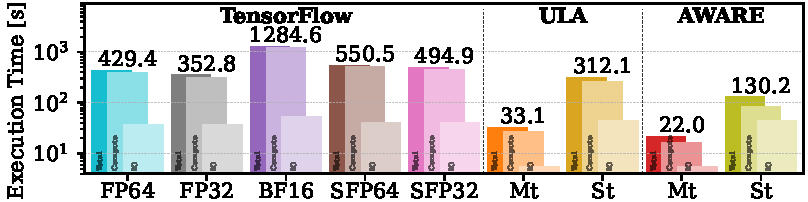
\includegraphics[width=0.8\linewidth]{\source/microbenchmark/comp/tensorflow_compare_dams-so001.pdf}
  \vspace{-0.25cm}
	\caption{\label{exp:tensorflow} TensorFlow Comparison {\normalfont(lmCG, US\,Census\,Enc)}.}
	\Description{TensorFlow compare}
\end{figure}


\textbf{Results:} Figure~\ref{exp:tensorflow} shows the results in log-scale, where each stack is I/O time,
compute time, and total time (from front to back, as regular stacking is infeasible in log scale).
On the left, we have TF with different value types.
Changing from FP64 (double) to FP32 improves execution time by 21.7\%, reducing to FP16 produces infinite sums, rendering the algorithm invalid.
BF16 solves this issue by using a different numbers of exponent and mantissa bits, but it is not well supported on the CPU,
resulting in a 3x slowdown compared to FP64.
Using TF's sparse representation worsen performance slightly at FP64 precision similarly at FP32.
TF executes the core expression per iteration (of two matrix-vector multiplications) $\mat{X}^{\top}(\mat{X}\,\mat{v})$ single-threaded because it only uses multi-threaded matrix multiplications with two or more columns in right-hand-side matrix.
In contrast, our multi-threaded I/O and matrix-vector multiplications yield speedups of about 13x for ULA and 19.5x for \name. 
Forcing both single-threaded I/O and operations (St), ULA becomes 38\% faster than TF.
ULA (with data size of $1.3\gb$) does not fully saturate the memory-bandwidth for this sparse dataset,
while \name~ fits the compressed matrix ($49.7\mb$) into the $128\mb$ L3 cache, yielding a 3.3x speedup over TF-FP64.
To summarize, both ULA and \name~ show competitive performance with single-threaded, and are faster with multi-threaded operations,
indicating that \name's improvements could carry over to other ML systems.

\subsection{Hyper-Parameter Tuning}

Executing a single short ML training algorithm makes it hard to amortize the online compression. In practice, however, most time is spent in ML pipelines that involve outer loops for enumerating data augmentation pipelines, feature and model selection, hyper-parameter tuning, and model debugging. \name\ adapts to such more complex workloads by spending more time on compression (which is easily amortized) and optimizing for operation performance in the inner loops. Table~\ref{tab:tabGridSearch} shows results for a basic GridSearch hyper-parameter tuning of the MLogReg algorithm. Even for a small number of $3\cdot3\cdot3\cdot5 = 90$ hyper-parameter configurations, \name~ improves the local runtime (including compression) by 3x, which is a promising result for wide practical applicability.

\begin{table} [!t] \setlength\tabcolsep{10pt}
	\centering
	\caption{\label{tab:tabGridSearch}GridSearch MLogReg (Data: US\,Census\,Enc).}
	\vspace{-0.4cm}
	\begin{tabular}{c|c|c}
\toprule
\textbf{ULA}       & \textbf{\name-Mem} & \textbf{\name}       \\
\midrule
\numprint{274.3} sec &	\numprint{238.1} sec &	\textbf{\numprint{92.6} sec}  \\
\bottomrule
\end{tabular}


\end{table}
